
%% bare_conf.tex
%% V1.3
%% 2007/01/11
%% by Michael Shell
%% See:
%% http://www.michaelshell.org/
%% for current contact information.
%%
%% This is a skeleton file demonstrating the use of IEEEtran.cls
%% (requires IEEEtran.cls version 1.7 or later) with an IEEE conference paper.
%%
%% Support sites:
%% http://www.michaelshell.org/tex/ieeetran/
%% http://www.ctan.org/tex-archive/macros/latex/contrib/IEEEtran/
%% and
%% http://www.ieee.org/

%%*************************************************************************
%% Legal Notice:
%% This code is offered as-is without any warranty either expressed or
%% implied; without even the implied warranty of MERCHANTABILITY or
%% FITNESS FOR A PARTICULAR PURPOSE!
%% User assumes all risk.
%% In no event shall IEEE or any contributor to this code be liable for
%% any damages or losses, including, but not limited to, incidental,
%% consequential, or any other damages, resulting from the use or misuse
%% of any information contained here.
%%
%% All comments are the opinions of their respective authors and are not
%% necessarily endorsed by the IEEE.
%%
%% This work is distributed under the LaTeX Project Public License (LPPL)
%% ( http://www.latex-project.org/ ) version 1.3, and may be freely used,
%% distributed and modified. A copy of the LPPL, version 1.3, is included
%% in the base LaTeX documentation of all distributions of LaTeX released
%% 2003/12/01 or later.
%% Retain all contribution notices and credits.
%% ** Modified files should be clearly indicated as such, including  **
%% ** renaming them and changing author support contact information. **
%%
%% File list of work: IEEEtran.cls, IEEEtran_HOWTO.pdf, bare_adv.tex,
%%                    bare_conf.tex, bare_jrnl.tex, bare_jrnl_compsoc.tex
%%*************************************************************************

% *** Authors should verify (and, if needed, correct) their LaTeX system  ***
% *** with the testflow diagnostic prior to trusting their LaTeX platform ***
% *** with production work. IEEE's font choices can trigger bugs that do  ***
% *** not appear when using other class files.                            ***
% The testflow support page is at:
% http://www.michaelshell.org/tex/testflow/



% Note that the a4paper option is mainly intended so that authors in
% countries using A4 can easily print to A4 and see how their papers will
% look in print - the typesetting of the document will not typically be
% affected with changes in paper size (but the bottom and side margins will).
% Use the testflow package mentioned above to verify correct handling of
% both paper sizes by the user's LaTeX system.
%
% Also note that the "draftcls" or "draftclsnofoot", not "draft", option
% should be used if it is desired that the figures are to be displayed in
% draft mode.
%
\documentclass[conference]{IEEEtran}
% Add the compsoc option for Computer Society conferences.
%
% If IEEEtran.cls has not been installed into the LaTeX system files,
% manually specify the path to it like:
% \documentclass[conference]{../sty/IEEEtran}
\usepackage{color}
\usepackage{amssymb}
\usepackage{algorithm}
\usepackage[noend]{algorithmic}

\usepackage{graphicx}
\DeclareGraphicsExtensions{.eps,.ps,.eps.gz,.ps.gz,.eps.Z}

\newcommand{\tabincell}[2]{\begin{tabular}{@{}#1@{}}#2\end{tabular}}
\IEEEoverridecommandlockouts

%% Use the option review to obtain double line spacing
%% \documentclass[authoryear,preprint,review,12pt]{elsarticle}

%% Use the options 1p,twocolumn; 3p; 3p,twocolumn; 5p; or 5p,twocolumn
%% for a journal layout:
%% \documentclass[final,1p,times]{elsarticle}
%% \documentclass[final,1p,times,twocolumn]{elsarticle}
%% \documentclass[final,3p,times]{elsarticle}
%% \documentclass[final,3p,times,twocolumn]{elsarticle}
%% \documentclass[final,5p,times]{elsarticle}
%% \documentclass[final,5p,times,twocolumn]{elsarticle}

%% For including figures, graphicx.sty has been loaded in
%% elsarticle.cls. If you prefer to use the old commands
%% please give \usepackage{epsfig}

%% The amssymb package provides various useful mathematical symbols
\usepackage{amssymb}
\usepackage{amsmath}
%% The amsthm package provides extended theorem environments
%% \usepackage{amsthm}




% Some very useful LaTeX packages include:
% (uncomment the ones you want to load)


% *** MISC UTILITY PACKAGES ***
%
%\usepackage{ifpdf}
% Heiko Oberdiek's ifpdf.sty is very useful if you need conditional
% compilation based on whether the output is pdf or dvi.
% usage:
% \ifpdf
%   % pdf code
% \else
%   % dvi code
% \fi
% The latest version of ifpdf.sty can be obtained from:
% http://www.ctan.org/tex-archive/macros/latex/contrib/oberdiek/
% Also, note that IEEEtran.cls V1.7 and later provides a builtin
% \ifCLASSINFOpdf conditional that works the same way.
% When switching from latex to pdflatex and vice-versa, the compiler may
% have to be run twice to clear warning/error messages.






% *** CITATION PACKAGES ***
%
%%\usepackage{cite}
% cite.sty was written by Donald Arseneau
% V1.6 and later of IEEEtran pre-defines the format of the cite.sty package
% \cite{} output to follow that of IEEE. Loading the cite package will
% result in citation numbers being automatically sorted and properly
% "compressed/ranged". e.g., [1], [9], [2], [7], [5], [6] without using
% cite.sty will become [1], [2], [5]--[7], [9] using cite.sty. cite.sty's
% \cite will automatically add leading space, if needed. Use cite.sty's
% noadjust option (cite.sty V3.8 and later) if you want to turn this off.
% cite.sty is already installed on most LaTeX systems. Be sure and use
% version 4.0 (2003-05-27) and later if using hyperref.sty. cite.sty does
% not currently provide for hyperlinked citations.
% The latest version can be obtained at:
% http://www.ctan.org/tex-archive/macros/latex/contrib/cite/
% The documentation is contained in the cite.sty file itself.






% *** GRAPHICS RELATED PACKAGES ***
%
\ifCLASSINFOpdf
  % \usepackage[pdftex]{graphicx}
  % declare the path(s) where your graphic files are
  % \graphicspath{{../pdf/}{../jpeg/}}
  % and their extensions so you won't have to specify these with
  % every instance of \includegraphics
  % \DeclareGraphicsExtensions{.pdf,.jpeg,.png}
\else
  % or other class option (dvipsone, dvipdf, if not using dvips). graphicx
  % will default to the driver specified in the system graphics.cfg if no
  % driver is specified.
  % \usepackage[dvips]{graphicx}
  % declare the path(s) where your graphic files are
  % \graphicspath{{../eps/}}
  % and their extensions so you won't have to specify these with
  % every instance of \includegraphics
  % \DeclareGraphicsExtensions{.eps}
\fi
% graphicx was written by David Carlisle and Sebastian Rahtz. It is
% required if you want graphics, photos, etc. graphicx.sty is already
% installed on most LaTeX systems. The latest version and documentation can
% be obtained at:
% http://www.ctan.org/tex-archive/macros/latex/required/graphics/
% Another good source of documentation is "Using Imported Graphics in
% LaTeX2e" by Keith Reckdahl which can be found as epslatex.ps or
% epslatex.pdf at: http://www.ctan.org/tex-archive/info/
%
% latex, and pdflatex in dvi mode, support graphics in encapsulated
% postscript (.eps) format. pdflatex in pdf mode supports graphics
% in .pdf, .jpeg, .png and .mps (metapost) formats. Users should ensure
% that all non-photo figures use a vector format (.eps, .pdf, .mps) and
% not a bitmapped formats (.jpeg, .png). IEEE frowns on bitmapped formats
% which can result in "jaggedy"/blurry rendering of lines and letters as
% well as large increases in file sizes.
%
% You can find documentation about the pdfTeX application at:
% http://www.tug.org/applications/pdftex





% *** MATH PACKAGES ***
%
%\usepackage[cmex10]{amsmath}
% A popular package from the American Mathematical Society that provides
% many useful and powerful commands for dealing with mathematics. If using
% it, be sure to load this package with the cmex10 option to ensure that
% only type 1 fonts will utilized at all point sizes. Without this option,
% it is possible that some math symbols, particularly those within
% footnotes, will be rendered in bitmap form which will result in a
% document that can not be IEEE Xplore compliant!
%
% Also, note that the amsmath package sets \interdisplaylinepenalty to 10000
% thus preventing page breaks from occurring within multiline equations. Use:
%\interdisplaylinepenalty=2500
% after loading amsmath to restore such page breaks as IEEEtran.cls normally
% does. amsmath.sty is already installed on most LaTeX systems. The latest
% version and documentation can be obtained at:
% http://www.ctan.org/tex-archive/macros/latex/required/amslatex/math/





% *** SPECIALIZED LIST PACKAGES ***
%
%\usepackage{algorithmic}
% algorithmic.sty was written by Peter Williams and Rogerio Brito.
% This package provides an algorithmic environment fo describing algorithms.
% You can use the algorithmic environment in-text or within a figure
% environment to provide for a floating algorithm. Do NOT use the algorithm
% floating environment provided by algorithm.sty (by the same authors) or
% algorithm2e.sty (by Christophe Fiorio) as IEEE does not use dedicated
% algorithm float types and packages that provide these will not provide
% correct IEEE style captions. The latest version and documentation of
% algorithmic.sty can be obtained at:
% http://www.ctan.org/tex-archive/macros/latex/contrib/algorithms/
% There is also a support site at:
% http://algorithms.berlios.de/index.html
% Also of interest may be the (relatively newer and more customizable)
% algorithmicx.sty package by Szasz Janos:
% http://www.ctan.org/tex-archive/macros/latex/contrib/algorithmicx/




% *** ALIGNMENT PACKAGES ***
%
%\usepackage{array}
% Frank Mittelbach's and David Carlisle's array.sty patches and improves
% the standard LaTeX2e array and tabular environments to provide better
% appearance and additional user controls. As the default LaTeX2e table
% generation code is lacking to the point of almost being broken with
% respect to the quality of the end results, all users are strongly
% advised to use an enhanced (at the very least that provided by array.sty)
% set of table tools. array.sty is already installed on most systems. The
% latest version and documentation can be obtained at:
% http://www.ctan.org/tex-archive/macros/latex/required/tools/


%\usepackage{mdwmath}
%\usepackage{mdwtab}
% Also highly recommended is Mark Wooding's extremely powerful MDW tools,
% especially mdwmath.sty and mdwtab.sty which are used to format equations
% and tables, respectively. The MDWtools set is already installed on most
% LaTeX systems. The lastest version and documentation is available at:
% http://www.ctan.org/tex-archive/macros/latex/contrib/mdwtools/


% IEEEtran contains the IEEEeqnarray family of commands that can be used to
% generate multiline equations as well as matrices, tables, etc., of high
% quality.


%\usepackage{eqparbox}
% Also of notable interest is Scott Pakin's eqparbox package for creating
% (automatically sized) equal width boxes - aka "natural width parboxes".
% Available at:
% http://www.ctan.org/tex-archive/macros/latex/contrib/eqparbox/





% *** SUBFIGURE PACKAGES ***
%\usepackage[tight,footnotesize]{subfigure}
% subfigure.sty was written by Steven Douglas Cochran. This package makes it
% easy to put subfigures in your figures. e.g., "Figure 1a and 1b". For IEEE
% work, it is a good idea to load it with the tight package option to reduce
% the amount of white space around the subfigures. subfigure.sty is already
% installed on most LaTeX systems. The latest version and documentation can
% be obtained at:
% http://www.ctan.org/tex-archive/obsolete/macros/latex/contrib/subfigure/
% subfigure.sty has been superceeded by subfig.sty.



%\usepackage[caption=false]{caption}
%\usepackage[font=footnotesize]{subfig}
% subfig.sty, also written by Steven Douglas Cochran, is the modern
% replacement for subfigure.sty. However, subfig.sty requires and
% automatically loads Axel Sommerfeldt's caption.sty which will override
% IEEEtran.cls handling of captions and this will result in nonIEEE style
% figure/table captions. To prevent this problem, be sure and preload
% caption.sty with its "caption=false" package option. This is will preserve
% IEEEtran.cls handing of captions. Version 1.3 (2005/06/28) and later
% (recommended due to many improvements over 1.2) of subfig.sty supports
% the caption=false option directly:
%\usepackage[caption=false,font=footnotesize]{subfig}
%
% The latest version and documentation can be obtained at:
% http://www.ctan.org/tex-archive/macros/latex/contrib/subfig/
% The latest version and documentation of caption.sty can be obtained at:
% http://www.ctan.org/tex-archive/macros/latex/contrib/caption/




% *** FLOAT PACKAGES ***
%
%\usepackage{fixltx2e}
% fixltx2e, the successor to the earlier fix2col.sty, was written by
% Frank Mittelbach and David Carlisle. This package corrects a few problems
% in the LaTeX2e kernel, the most notable of which is that in current
% LaTeX2e releases, the ordering of single and double column floats is not
% guaranteed to be preserved. Thus, an unpatched LaTeX2e can allow a
% single column figure to be placed prior to an earlier double column
% figure. The latest version and documentation can be found at:
% http://www.ctan.org/tex-archive/macros/latex/base/



%\usepackage{stfloats}
% stfloats.sty was written by Sigitas Tolusis. This package gives LaTeX2e
% the ability to do double column floats at the bottom of the page as well
% as the top. (e.g., "\begin{figure*}[!b]" is not normally possible in
% LaTeX2e). It also provides a command:
%\fnbelowfloat
% to enable the placement of footnotes below bottom floats (the standard
% LaTeX2e kernel puts them above bottom floats). This is an invasive package
% which rewrites many portions of the LaTeX2e float routines. It may not work
% with other packages that modify the LaTeX2e float routines. The latest
% version and documentation can be obtained at:
% http://www.ctan.org/tex-archive/macros/latex/contrib/sttools/
% Documentation is contained in the stfloats.sty comments as well as in the
% presfull.pdf file. Do not use the stfloats baselinefloat ability as IEEE
% does not allow \baselineskip to stretch. Authors submitting work to the
% IEEE should note that IEEE rarely uses double column equations and
% that authors should try to avoid such use. Do not be tempted to use the
% cuted.sty or midfloat.sty packages (also by Sigitas Tolusis) as IEEE does
% not format its papers in such ways.





% *** PDF, URL AND HYPERLINK PACKAGES ***
%
%\usepackage{url}
% url.sty was written by Donald Arseneau. It provides better support for
% handling and breaking URLs. url.sty is already installed on most LaTeX
% systems. The latest version can be obtained at:
% http://www.ctan.org/tex-archive/macros/latex/contrib/misc/
% Read the url.sty source comments for usage information. Basically,
% \url{my_url_here}.





% *** Do not adjust lengths that control margins, column widths, etc. ***
% *** Do not use packages that alter fonts (such as pslatex).         ***
% There should be no need to do such things with IEEEtran.cls V1.6 and later.
% (Unless specifically asked to do so by the journal or conference you plan
% to submit to, of course. )


% correct bad hyphenation here
%%\hyphenation{op-tical net-works semi-conduc-tor}


\begin{document}
%
% paper title
% can use linebreaks \\ within to get better formatting as desired
\title{CPCR: Contact-Prediction Clustering-based Routing \\in Large-scale Urban Vehicular Delay Tolerant Networks}


% author names and affiliations
% use a multiple column layout for up to three different
% affiliations
\author{\IEEEauthorblockN{Wenjing Yang}
\IEEEauthorblockA{School of Software\\Beihang University\\
Beijing, P.R.China\\
Email: yangwenjing@sse.buaa.edu.cn}
\and
\IEEEauthorblockN{Haiquan Wang\thanks{
 This research has been partially supported by the US National Science Foundation (NSF) under Grant No. CNS-1319915 and CNS-1343355, the National Natural Science Foundation of China (NSFC) under Grant No.61300173 and No. 61170295, the Project of Aeronautical Science Foundation of China under Grant No.2013ZC51026 and No.2011ZC51024, the Fundamental Research Funds for the Central Universities under Grant No. YWF-12-LXGY-001, and the State Key Laboratory Software Development Environment and Network Information and Computing Center of Beihang University.
}}
\IEEEauthorblockA{School of Software\\Beihang University\\
Beijing, P.R.China\\Beijing Key Laboratory of\\Network Technology
Beijing, P.R.China\\
Email: whq@buaa.edu.cn}
\and
\IEEEauthorblockN{Jingtao Zhang\\ and Jiejie Zhao}
\IEEEauthorblockA{School of Software\\Beihang University\\
Beijing, P.R.China\\
Email: zjt@buaa.edu.cn\\Email: zjj@buaa.edu.cn}}

% conference papers do not typically use \thanks and this command
% is locked out in conference mode. If really needed, such as for
% the acknowledgment of grants, issue a \IEEEoverridecommandlockouts
% after \documentclass

% for over three affiliations, or if they all won't fit within the width
% of the page, use this alternative format:
%
%\author{\IEEEauthorblockN{Michael Shell\IEEEauthorrefmark{1},
%Homer Simpson\IEEEauthorrefmark{2},
%James Kirk\IEEEauthorrefmark{3},
%Montgomery Scott\IEEEauthorrefmark{3} and
%Eldon Tyrell\IEEEauthorrefmark{4}}
%\IEEEauthorblockA{\IEEEauthorrefmark{1}School of Electrical and Computer Engineering\\
%Georgia Institute of Technology,
%Atlanta, Georgia 30332--0250\\ Email: see http://www.michaelshell.org/contact.html}
%\IEEEauthorblockA{\IEEEauthorrefmark{2}Twentieth Century Fox, Springfield, USA\\
%Email: homer@thesimpsons.com}
%\IEEEauthorblockA{\IEEEauthorrefmark{3}Starfleet Academy, San Francisco, California 96678-2391\\
%Telephone: (800) 555--1212, Fax: (888) 555--1212}
%\IEEEauthorblockA{\IEEEauthorrefmark{4}Tyrell Inc., 123 Replicant Street, Los Angeles, California 90210--4321}}




% use for special paper notices
%\IEEEspecialpapernotice{(Invited Paper)}




% make the title area
\maketitle


\begin{abstract}
%\boldmath
Routing in Public Transport Networks is particularly challenging due to the high mobility, rapidly changing topology. Though clustering of nodes can aid forwarding decision in these Delay Tolerant Networks (DTNs), centralized clustering process is extremely costly in a large network. Moreover, it is critical to choose proper metrics to cluster nodes. In this paper, we propose a contact-predict clustering-based routing algorithm, CPCR, for large-scale urban DTNs. This algorithm computes the probability for each node pair and cluster that nodes distributively into higher contact-strength clusters using nodal local contact information. Depending on the clusters, intra-cluster and inter-cluster routing strategies will be adopted. Extensive simulations indicate that CPCR maintains relatively stable clusters and enhances the routing performance. The results demonstrate that clustering-based routing algorithm is rational and promising for large-scale urban DTNs.
\end{abstract}
% IEEEtran.cls defaults to using nonbold math in the Abstract.
% This preserves the distinction between vectors and scalars. However,
% if the conference you are submitting to favors bold math in the abstract,
% then you can use LaTeX's standard command \boldmath at the very start
% of the abstract to achieve this. Many IEEE journals/conferences frown on
% math in the abstract anyway.

% no keywords
\begin{IEEEkeywords}
clustering,  inter-contact time ,contact prediction ,delay tolerant networks
\end{IEEEkeywords}




% For peer review papers, you can put extra information on the cover
% page as needed:
% \ifCLASSOPTIONpeerreview
% \begin{center} \bfseries EDICS Category: 3-BBND \end{center}
% \fi
%
% For peerreview papers, this IEEEtran command inserts a page break and
% creates the second title. It will be ignored for other modes.
\IEEEpeerreviewmaketitle



\section{Introduction}
\label{INTRODUCTION}
% no \IEEEPARstart
Delay Tolerant Networks (DTNs) \cite{aFall-2,cAhmedSalil-4} is a branch of networks,
where communication links only exist temporarily with a highly dynamic topology. One of such examples is vehicular network, in which, vehicles communicate with each other in order to disseminate data using opportunistic contacts.

Traditional flat routing methods, such as \emph{Direct Delivery} (DD) \cite{eKleywegtNori-6} and \emph{Epidemic Routing} \cite{gVahdatBecker-8}, become not scalable to large-scale DTNs. Meanwhile, clustering-based approaches have long been considered as an effective approach to reduce network overhead and improve scalability in traditional mobile ad hoc networks \cite{hAgarwalMotwani-9,iLiuLiu-10,jWangMi-11,kWhitbeckConan-12} with relatively stable topology and more communication opportunity.
Clustering in DTNs is unique \cite{uHaHongyi-22,kernal2005survey}, because the network topology is not always fully connected. As a result, it becomes much more challenging to formulate clusters and ensure their stability. When we consider an urban DTN, the nodal scale and mobility will further increase the cost of maintaining clusters.

Contact characteristics among nodes \cite{nGaoCao-15,oWhitbeckConan-16,p20102413007279} have been used as one of key metrics for clustering in DTNs. Frequency and duration of historical contacts have been used as metrics to describe contact probability \cite{rLiHui-19,t20102413006168}, however they cannot provide very accurate estimation of the contact probability among nodes. Instead, the distribution of  \emph{inter-contact time} (ICT) has been shown to be powerful for describing contact characteristics \cite{rLiHui-19,qGroeneveltNain-18,s20104613388174}. ICT between two nodes directly affects the transmission delay between these two nodes, since a shorter ICT implies a greater opportunity to relay packet in a period of time.

In this paper, we propose an clustering-based routing scheme for large-scale urban DTNs.  We first
analyze a real-world urban vehicular tracing data set to reveal the Inter-contact time distributions of mobile vehicles in a large city. Our study confirm that both the global ICT and the individual ICT between each nodal pair follow the exponential distributions.
It is demonstrated that the distribution for ICT of nodal pairs is more accuracy than the global ICT distribution. Therefore, a clustering algorithm which groups nodes by the contact probability calculated from the ICT distribution for nodal pair in real-time, and propose a new clustering-based routing scheme based on this contact predication clustering.

To summarize, our contributions in this paper can be highlighted as follows:
    \begin{itemize}
      \item
         Via an in-depth analysis of the Beijing taxi data set, we demonstrate that it is applicable to estimate the parameter for the ICT exponential distribution of every nodal pair. Such pair-wise ICT distribution is more accurate then the global ICT distribution, which is commonly used in several DTN routing schemes.
      \item
         A hierarchical routing algorithm, CPCR, based on a distributed clustering via contact prediction is proposed.  CPCR uses direct delivery and flooding strategy in intra-cluster and inter-cluster routing phases, respectively.
      \item %%evaluation
        Extensive simulations are conducted with the Beijing taxi tracing data to evaluate the efficiency and scalability of the proposed clustering-based routing.
    \end{itemize}

The rest of paper is organized as follows: Section \ref{Section2_relatedwork} provides an overview of related work on DTN routing.
Section \ref{Section3_characteristics} provides the theoretical basis of contact predicting and clustering via detailed analysis of the Beijing taxi traces. Section \ref{Section4_algorithm} presents our clustering-based routing algorithm which leverages the estimated ICT distributions to clustering nodes into groups and routes the packages accordingly. Simulation results over the Beijing taxi traces are presented in Section \ref{Section6_simulation}. Finally, Section \ref{Section6_conclusions} concludes this paper.


\section{Related Work}
\label{Section2_relatedwork}

In 2004, Jain et al. \cite{JainFall-771} first investigate the routing issues in DTNs, where messages are to be moved
end-to-end across a graph that is time-varying and not full connected. Since then routing in DTNs has been heavily studied \cite{cao2013routing,ZXSW13-DTN-survey} over the last decade.
Routing algorithms can be categorized into \emph{flat routing} or \emph{hierarchical routing} by the network topology.
Flat routing methods employ only a single routing strategy globally, while all nodes play similar roles. For example,
\emph{Epidemic Routing} \cite{VahdatBecker-779} is a simple flooding method with zero knowledge of the network topology.  Compared with some single-copy routing methods, such as \emph{Direct Delivery} \cite{BalasubramanianLevine-489}, \emph{Randomized Routing} (RR) \cite{LeightonMaggs-780},  Epidemic routing greatly improves delivery ratio but suffers from resource waste and even network congestion due to large data replication. In order to reduce the usage of resources, \emph{Spray and Wait} routing \cite{SpyropoulosPsounis-772} limits the amount of message copies in its spray phrase and lets node wait until contacted by the destination node in its wait phrase. But with such solutions, routing performance could still be poor in large-scale networks.
Besides these flooding based schemes \cite{VahdatBecker-779,GrossglauserTse-777,SpyropoulosPsounis-778}, there is also a set of DTN routing methods based on the contact information, where a smarter relay node selection is made \cite{LindgrenDoria-782,BurgessGallagher-783}.
For example, \emph{PRoPHET} is a probability-based method, where each node maintains the encounter history.

When the network scale increases and topology evolves, however, the scalability and performance of flat routing methods are limited.
Under this condition, hierarchical routing organizes the networks in groups via clustering techniques. It has been shown that hierarchical routing can achieve good scalability in large-scale mobile networks. However, restricted by the dynamic topology and frequently interruptions, hierarchical routing in DTNs is still in its early stages. Liu and Wu \cite{lLiuWu-1103} design a hierarchical DTN routing algorithm based on a strict mobility model, where all nodes move according to strict repetitive patterns. Their method is only effective such a specific mobility model and could not adapt to other mobility pattern. Ahmed and Kanhere \cite{mAhmedKanhere-14} adopt encounter frequencies of public transport networks to classify nodes. Nodes only relay messages to neighboring nodes which are in the same cluster of the destination node. Then epidemic routing is used to propagate messages inside the cluster.
These clustering-based hierarchical routing methods can improve the scalability, but the resource consumption of collecting and maintaining historical information remains high.
 a hybrid DTN-MANET (HYMAD) routing was proposed by Whitbeck and Conan \cite{oWhitbeckConan-16} for dense and highly dynamic wireless networks.
This method is decentralized and only makes use of topological information exchanges between the nodes, thus limit the storage and information exchange cost. However,  its intra-cluster routing using MANET method may be invalid. It can not suit for more complicated urban DTNs.

In summary, the key challenge of hierarchical routing is the clustering method, especially in large scale DTNs. To adapt to the scenario of large scale urban DTNs and solve the routing problem, a cluster-based routing algorithm is proposed.

\section{Characteristics of Large-scale Urban DTNs}
\label{Section3_characteristics}

In this section, we mainly focus on revealing the inherent characteristics of contacts and possible clustering methods in large-scale urban DTNs by analyzing a real-world trace data. We believe that these are essential properties which affect DTN routing design and verification.


\subsection{Trace Dataset: Beijing Taxi Traces}
\label{Trace Data}

To study urban DTNs, we use a real-world GPS dataset  which were generated by $12,096$ taxis in Beijing, China within one week (from June 13th to 19th, 2010). This dataset has been used by several key research and application programs of Intelligent Transportation Systems (ITS) in Beijing, China. The number of participated taxis ($12,096$ taxis) is $18\%$ of the total taxis in the city. Each taxi is equipped with a GPS device and upload its information (including location, speed, direction, et al. ) about every 60 seconds. There are around $1.22 \times 10^8$ records in total.
For each row, the record includes a base station ID, company name, taxi ID ($id$), timestamp ($t$), current location ($l$, including both longitude and latitude), another location (out of $54$ fixed locations), speed, acceleration, status of the taxi, event, and height. Out of this information, we only use the taxi ID, timestamp, and current location, i.e., $(id,t,l)$,  to generate the contacts among taxis for the study within this paper.  Notice that GPS traces from taxis have been used recently for inferring human mobility \cite{Ganti:2013:IHM:2493432.2493466} and modelling city-scale traffics \cite{Aslam:2012:CTE:2426656.2426671}. Therefore, we believe that they are also suitable to characterize the contact patterns among vehicles in large-scale urban DTNs.

\subsection{Contact Characteristics in Beijing Taxi Traces}
\label{Contact Characteristics}

The \emph{inter-contact time} (ICT) is the interval time between two continuous contacts for same nodal pair. ICT implies the contacts frequency of two nodes. Researchers have focused on the study of ICT characteristics for different mobility patterns in DTNs, and lead to numerous ICT distribution results of both theoretical and real-world mobility models. Most ICT distribution models are created as exponential distributions. According to \cite{qGroeneveltNain-18,vHuWang-23,yJiangLi-26} , the ICT between two mobile nodes generates exponential distributions where the exponential parameter is related to the motion characteristics. Simulations in \cite{qGroeneveltNain-18,z20102212975997} based on random waypoint and random direction mobility models confirm such claims.
In the real-world mobility traces of vehicular networks \cite{zaZhuLi-28}, the ICT between two vehicles also follows an exponential distribution.Similar conclusions have been found in another Shanghai taxi trace dataset studied by  \cite{zaZhuLi-28,zb20080311017302}. The contact probability between any two nodes based on the global ICT distribution is
 \begin{equation}
    P(X>x)=e^{-\lambda t},
 \end{equation}
where the exponential parameter $\lambda$ reflects the contact strength between nodes. A static $\lambda$ can be estimated for the whole network by fitting the global ICT distribution to the exponential function. This simple method can measure the contact strength intuitively and efficiently, and has been frequently used in many DTN routing methods.

 Paper \cite{vHuWang-23} studied the ICT distributions of individual nodal pairs and find that they follow exponential distributions under three assumptions. The ICT of a node pair $i$ and $j$ also follows the exponential distribution with exponential parameters $\lambda_{ij}$, according to:
 \begin{equation}\label{equation_label_lambda}
        \lambda_{ij} = n_{ij}/\sum ICT_{ij},
 \end{equation}
where $n_{ij}$ refers to the number of contacts between nodes $i$ and $j$, and $\sum ICT_{ij}$ indicates the total ICTs between these two nodes. Hence, the contact probability of nodes $i$ and $j$ within time period $t$ is
\begin{equation}\label{equation_label_probability}
    p_{ij}(t)=P_{ij}(X\leq t)= 1-e^{-{n_{ij}\over {\sum ICT_{ij}}}t}.
 \end{equation}

\begin{figure}[!h]
\centering
  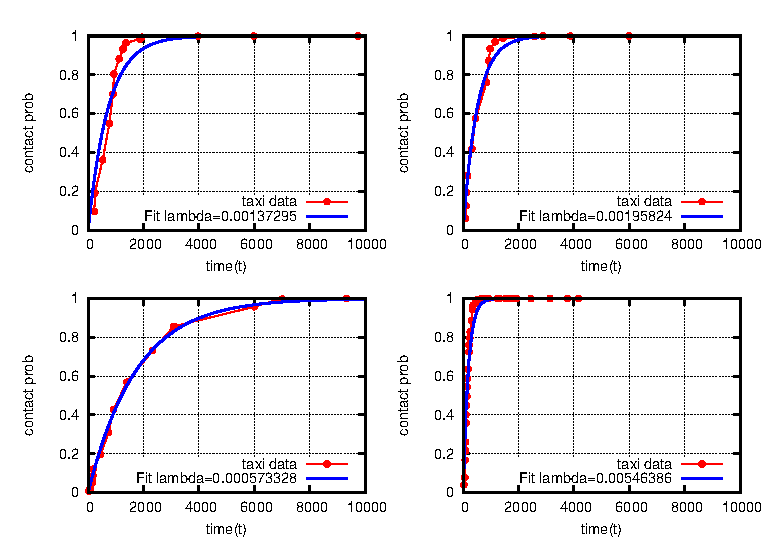
\includegraphics[width=3.5in]{figures_1/multiplot-nodepair.eps}
  \caption{Pairwise ICT distributions of four nodal pairs in Beijing taxi dataset. Red dots are the real sample data from the dataset while blue curves are the fitted exponential distributions.}\label{figure_label_ICT_Distribution}
\end{figure}

By fitting the samples of ICTs for a particular nodal pair with Equation \ref{equation_label_lambda}, we can derive the exponential parameters $\lambda_{ij}$. The values of $\lambda_{ij}$ in Beijing taxi dataset varies significantly from $0.0005$ to $0.005$. Figure \ref{figure_label_ICT_Distribution} shows the exponential distributions fitting for four pairs of nodes.

To further confirm that the method based on pair-wise ICT distributions can characterize the real contact pattern better than the aggregated global ICT distribution, we also use the coefficient of determination $R^{2}$ \cite{ozer1985correlation} to determine the similarity degree of modelled ICT curves and real observed curves from dataset. Note that $R^{2}$ is a number between $0$ and $1.0$, and used to describe how well a regression line fits a set of data. An $R^{2}$ near $1.0$ indicates that a regression line fits the data perfectly, while an $R^{2}$ closer to $0$ indicates that a regression line does not fit the data very well.

\begin{figure}[!h]
\centering
  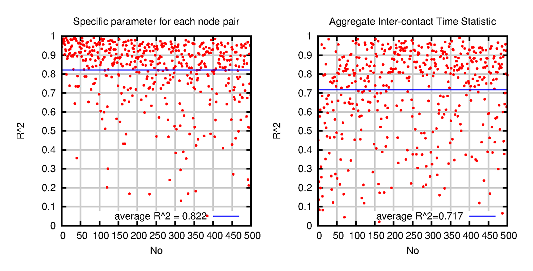
\includegraphics[width=3.5in]{figures_1/R2_comprision.eps}\\
  (a) the pair-wise ICT method \ \ \ \ \ \ \ \ \ \ \ \ \ (b) the global ICT method
  \caption{Comparison of similarities $R^2$ of the two estimation methods. Here, red dots are the values of $R^2$ for $500$ node pairs, while the blue line shows the average value of these $R^2$.}\label{figure_label_Comparison_between_R2}
\end{figure}

For the global ICT method,  we attract the $\lambda$ based on all contact records, and result $\lambda= 0.00077527$. For the pair-wise ICT method, we use Equation  \ref{equation_label_lambda} to learn the individual $\lambda_{ij}$ for each nodal pair. Then we calculate  $R^{2}$  between the estimated distributions based on $\lambda$ or $\lambda_{ij}$ with the real distributions from traces of individual nodal pairs in the dataset. Figure \ref{figure_label_Comparison_between_R2} shows plots of such comparison over  $500$ randomly generated nodal pairs. Clearly, $R^{2}$ differs for each pair of nodes. The blue line in both plots are the average $R^{2}$. The global ICT method has an average of $R^{2}$ at $0.717$ while the pair-wise one is $0.822$. This confirm that using pair-wise ICT distribution can fit the real records better and thus give better contact probability over the global fitting method. Therefore, in our proposed clustering method, we use a distributed algorithm to estimate $\lambda_{ij}$ for every nodal pair.

\section{Routing based on Clusters}
\label{Section4_algorithm}

Now we are ready to describe the proposed \emph{Contact-Prediction Clustering-based Routing} method (CPCR).
CPCR leverages the estimated pair-wise ICT distribution (via Equation \ref{equation_label_lambda}) to predict the contact probability among nodes (using Equation \ref{equation_label_probability}), and uses such probabilities to form clusters. Based on the clustering,
CPCR perform its intra- and inter-cluster routing strategies, respectively.

\subsection{Data Structure and Notations}
We first review basic data structures and notations in CPCR. The following data structures are used at each node.
 \begin{align*}
        \left\{
        \begin{array}{l}
            Node = \tabincell{l}{(id, cid, ContactTable, GatewayTable,\\ConnectionList, MessageList, timer)}\\
            ContactTable = \{ContactRecord_1,\cdots, ContactRecord_n\}\\
            GatewayTable = \{GatewayRecord_1,\cdots, GatewayRecord_m\} \\
            ConnectionList=\{Connection_1,\cdots, Connection_o\}\\
            MessageList = \{MassageRecord_1, \cdots,MassageRecord_p\}\\
            ContactRecord = (id, cid, contactTimes, \sum ICT, contactProb, timestamp)\\
            GatewayRecord = (cid, gid, timeout)\\
            MessageRecord = (message, FloodingClusters)\\
            Connection = (remoteEndNode, message)\\
        \end{array}
        \right.
    \end{align*}
Table \ref{detal_data_structure} gives all notations used here.
\begin{table}[!h]
    \caption{Notations used in our data structure.}\label{detal_data_structure}
    \vspace{.1in}
    \begin{tabular}[c]{r|l}
    \hline
    \textbf{Symbol} & \textbf{Description} \\
    \hline
    $id$ & unique identifier of a node\\
    $gid$ & unique identifier of gateway node $id$ to another cluster\\
    $cid$ & unique identifier of cluster which contains the node\\
    $ContactTable$ & a table stores contact records\\
    $GatewayTable$ & a table stores gateway records\\
    $ConnectionList$& stores all established connections\\
    $MessageList$ & stores messages and their historical info\\
    $timer$ & to remind nodes of periodic updating\\
   \hline
    $ContactRecord$  & contacts to other nodes and their contact-probability\\
    $GatewayRecord$ & gateway nodes info, with a timer\\
    $Connection$ & message information and the other contacting node\\
    $remoteEndNode$ & the other contacting node\\
    $message$ & data needs to transmit\\
    $FloodingClusters$ & a collection of clusters with the message copy\\
    $contactTimes$ & contact times between two nodes\\
    $timestamp$ & time record, when connection is up or down\\
    $\sum ICT$ or $\sum ICT_{ij}$ & total ICT between two nodes ($i$ and $j$)\\
    $contactProb$ & contact probability between nodes\\
    $timeout$ & a timestamp to decide whether a record expires\\
    \hline
    \end{tabular}
\end{table}

\subsection{Clustering Criteria}
\label{section_label_clustering_criterion}
CPCR utilizes $p_{ij}(t)$, contact probability for nodes $i$ and $j$ in time period $t$, as the clustering metric, since it implies contact strength between the two nodes. Hereafter, $p_{ij}(t)$ can be simplified as $p_{ij}$. The clustering criteria is given as follows:
\begin{description}
  \item[Criterion 1] We group nodes with contact probability higher than a probability threshold $\eta$ into clusters.
  \item[Criterion 2] If a node conforms with the Criterion 1 for two or more clusters, the node will join the most stable cluster.
\end{description}
Accordingly, a cluster can be represented as a collection of nodes as follows:
    \begin{equation}\label{equation_collections}
          C= \{ ID_{k} | k=1,2,\dots,n;\forall i,j\in \{1,2,3,\dots,n\},p_{ij}(t)>\eta\}.
    \end{equation}
Assume based on Criterion 1 node $i$ belongs to two cluster $C_m$ and $C_n$, i.e., $p_{ij}>\eta, p_{ik}>\eta$ for ${\forall j,k, j \in C_m, k \in C_n}$.  In this case, we use the minimum contact probability in a cluster to represent the stability of that cluster. By comparing $\min(p_{m_1m_2})$ and $\min(p_{n_1n_2})$, $\forall m_1,m_2 \in C_m$ and $\forall n_1,n_2 \in C_n$, node $i$ will join the cluster with higher minimum probability.

Note that two parameters $t$ and $\eta$ can affect the contact probability and thus affect the results of clustering. When $\eta$ is a constant, a smaller $t$ decreases $p_{ij}(t)$ so that fewer nodes will meet the clustering criterion. Thus, smaller but more stable
clusters will be generated. As a consequence, the overhead of intra-cluster routing and clustering maintenance will decrease whereas the overhead of inter-cluster routing will increase. On the other hand, increasing $\eta$ can increase the contact strength in clusters and guarantee the efficiency of intra-cluster routing, whereas, more clustering fragments will occur. Overall, reasonable values of $t$ and $\eta$ need to be configured for tradeoff between clustering and routing.



\subsection{Distributed Clustering  based on Contact Perdiction}
\label{section_label_clustering_procedure}

CPCR use the above clustering criteria to perform the clustering among mobile nodes.  The assumption that the network topology remains static in the initial clustering phase in MANET applications, does not apply to DTNs where nodes move randomly over time.
Therefore, the clustering algorithm in DTNs should be distributed, heuristic and self-maintaining. In CPCR, nodes cooperatively execute the clustering algorithm and communicate with other nodes. The concept of cluster head, which acts as a coordinator in most clustering designs, is not introduced in CPCR. In our opinion, nodes are homogeneous because of their similar communication and computation abilities in DTNs. Moreover, it is difficult to avoid redundant bottlenecks when routing with cluster heads.
The detailed overall clustering method is given in Algorithm \ref{algorithm_clustering} which includes information exchange upon contact, periodic updating of $ContactTable$ and $GatewayTable$, and deleting related gateway records when they expire.

\begin{algorithm}[!t]
\caption{Clustering Algorithm}\label{algorithm_clustering}
\begin{algorithmic}
\STATE \textbf{Initialization:} $timer \Leftarrow CurrentTime$,\\
$ContactTable \Leftarrow NULL$, \\$GatewayTable \Leftarrow  NULL$, $cid \Leftarrow id$
\WHILE{$Simulation \neq end$}
    \IF{Contacting}
        \STATE Contacting()
    \ELSE[$CurrentTime - timer > t$]
        \STATE Period-Updating()
        \FORALL{$GatewayRecord \in GatewayTable$}
            \IF{GatewayRecord.isTimeout}
                \STATE $GatewayTable.remove(GatewayRecord)$
            \ENDIF
        \ENDFOR
        \STATE $timer \Leftarrow CurrentTime $
    \ENDIF
\ENDWHILE
\end{algorithmic}
\end{algorithm}

\smallskip
\textbf{Initialization:} Initially, each node generates a cluster only including itself. The node also sets $ContactTable$ and $GatewayTable$ empty.

\smallskip
\textbf{Happen to Contact:} When two nodes move into each other's communication range, two nodes will execute the process shown in Algorithm \ref{algorithm_contacting}.

\begin{algorithm}[!t]
\caption{Contacting}\label{algorithm_contacting}
\begin{algorithmic}
\FORALL{$Connection \in ConnectionsList$}
\STATE $OtherNodes \Leftarrow Connection.remoteEndNode$
\STATE $ContactRecord \Leftarrow ContactTable[OtherNodes]$
\IF{$Connection = established$}
\STATE $ContactRecord.\sum ICT += CurrentTime-ContactRecord.timestamp$
\STATE $ContactRecord.contactTimes++$
\STATE $ContactRecord.contactProb =1-\exp\{-\frac{ContactRecord.contactTimes}{ContactRecord.\sum ICT}t\}$
\IF{$cid=OtherNodes.cid$}
\STATE $isBetterGateway(OtherNodes)$
\ELSE[$cid \neq OtherNodes.cid$]
\STATE $whetherToJoinOtherCluster(OtherNodes)$
\ENDIF
\ELSE[$Connection = destoried$]
\STATE $ContactRecord.timestamp = CurrentTime$
\ENDIF
\ENDFOR
\STATE Gateway-Updating()
\end{algorithmic}
\end{algorithm}

First, the cluster information of the other node is required. Upon contacting with node $j$, node $i$ will add or update the contact record with node $j$ and re-calculate the contact probability with node $j$ by Equation \ref{equation_label_probability}.
If $cid_i=cid_j$, node $i$ add or update the record in $GatewayTable_{i}$. Node $i$ will decide whether or not node $j$ can be a better gateway to cluster $cid_m$, when $cid_m \neq cid_j$, as follows:
\begin{enumerate}
      \item Node identifies the maximum contact probability to cluster $cid_j$ in $ContactTable_j$, which is denoted as:
\begin{center}
    $p_j^{cid_m}=MAX\left\{
    p_{jk}|\forall k,cid_k=cid_m
    \right\}$.
\end{center}
      \item  If $p_{ij}\times p_j^{cid_m}>p_{i,gid_i^{cid_m}}\times p_i^{cid_m}$, node j can be a better gateway for node $i$ to cluster $cid_m$, node $i$ will update the relevant record and reset the gateway timeout.
      \item In case that node $i$ has no gateway to cluster $cid_m$, node j will be set as the gateway only if node $j$ has any record which belongs to cluster $cid_m$.
    \end{enumerate}
If $cid_i \not= cid_j $ (i.e., $i$ and $j$ belong to different clusters), node $i$ will decide whether to join cluster $cid_j$.
The function $whetherToJoinOtherCluster(OtherNodes)$ are decided by criteria given in Section \ref{section_label_clustering_criterion}.

\smallskip
\textbf{Periodic Updating:}
To obtain a more precise real-time prediction, the algorithm needs to regularly update the records in $ContactTable$ and $GatewayTable$. The periodic record updating procedure is shown in Algorithm \ref{algorithm_period_updating}.

\begin{algorithm}[!t]
\caption{Period-Updating}\label{algorithm_period_updating}
\begin{algorithmic}
\FORALL{$ContactRecord \in ContactTable$}
\STATE $ContactRecord.contactProb =1-\exp\{-\frac{ContactRecord.contactTimes}{ContactRecord.\sum ICT}t\}$
\ENDFOR
\FORALL {$ContactRecord.cid == node.cid$}
\STATE $FLAG \Leftarrow \TRUE$
\IF{$ContactRecord.contactProb < \eta$}
\STATE $FLAGE \Leftarrow \FALSE$, $Break$
\ENDIF
\IF{$FLAG = \FALSE$}
\STATE $Node.cid \Leftarrow newClusterID()$
\STATE $Node.GatewayTable \Leftarrow NULL$
\ELSE
\STATE $Gateway-Updating()$
\ENDIF
\ENDFOR
\end{algorithmic}
\end{algorithm}

First, the local node $i$ updates $p_{ij}$ in $ContactTable_i$ with the latest $contactTimes$ and $\sum ICT$.
Then, it will go through clustering criteria check. If the node passes Criterion 1, it will remain in the original cluster.
Updating $ContactTable$ may change node $i$'s probability to the other clusters. Therefore, node $i$ will also update $GatewayTable_i$ to set the new or better gateway to other clusters. The gateway in $GatewayTable_i$ must in the same
cluster of node $i$. If the node does not pass Criterion 1, it will leave its original cluster and construct a new isolated cluster
which only includes itself. In such a situation, the node will keep its own $ContactTable$, while $GatewayTable$ will be set empty, since the old gateway records are meaningless to the new established cluster.

\subsection{Clustering-based Routing Scheme}
\label{section_label_routing_procedure}
Based on dynamically formed clusters, our clustering-based routing procedure can be divided into intra- and inter cluster routing procedures. If destination node is in the same cluster of a node, a single-copy routing strategy will be executed as intra-cluster routing algorithm. The local node will not deliver the packet until contacted by the destination node. Considering high contact probability inside a cluster, such direct delivery can simplify route decision making and ensure acceptable delay in the intra-cluster routing.
If the local node and the destination belong to the different clusters, inter-cluster flooding approach will be used. Every cluster is considered as an abstract "node". Therefore, it ensures that a cluster can only accept no more than one copy of a message.
Since CPCR is event-driven, the routing procedure will be executed when contacts happen. When node $i$ contacts with node $j$, node $i$ will traverse every message to determine whether or not to relay the messages. The routing procedure can be described as Algorithm \ref{algorithm_routing_procedure}.

 %%Routing after Contacting
\begin{algorithm}
\caption{Clustering-based Routing}\label{algorithm_routing_procedure}
\begin{algorithmic}
    \IF{$Connection = established$}
        \STATE $remoteNode \Leftarrow Connection.remoteNode$
        \FORALL{$message \in MassageList$}
            \STATE $destination \Leftarrow message.destination$
            \IF{$destination = remoteNode$}
                \STATE $sendAndDelete(message)$, CONTINUE
            \ENDIF
            \IF{$belongToSameCluster(this, destination)$}
                \STATE CONTINUE
           \ENDIF
            \IF{$belongToSameCluster(destination,remoteNode)$}
                \STATE $sendAndDelete(message)$
            \ELSE[$belongToSameCluster(this,remoteNode)$ ]
                \IF{$isGateway(remoteNode,destination.cid)$}
                   \STATE $sendAndDelete(message)$
                \ENDIF
            \ELSE
                \STATE $copyAndDelete(message)$
             \ENDIF
        \ENDFOR
    \ENDIF
\end{algorithmic}
\end{algorithm}

If the message's destination is node $j$,  node $i$ will send the message to node $j$. Then, the message will be deleted (as $sendAndDelete(message)$). If the destination of the message is in the same cluster of local node, message will not be relayed until the local node meets the destination node, which can be considered as intra-cluster routing. For inter-cluster routing where the remote node $j$ is not the destination and not in the same cluster of the local node, node $j$ can be a relay point if it satisfies one of following circumstances:
\begin{enumerate}
      \item The target cluster of the message is the same as the cluster of node $j$.
      \item The node $j$ is the gateway node from the cluster of node $i$ to the target cluster. As the definition for gateway, we can figure out that node $j$ belongs to the same cluster as the local node.
      \item Three nodes ($i$, $j$, and the destination node) belong to three different clusters. In this case, local node will send a copy to the remote node, only if there is no copy in the cluster of node $j$. When message has been sent, node $i$ will store a record that the $cluster_j$ has a copy of the message, avoid of sending a message to the same cluster again.
\end{enumerate}

Whether two nodes are in the same cluster is determined by exploring the $ContactTable$ and $GatewayTable$ of the local node. If we can neither find a record for a destination in $ContactTable$, nor find a gateway to the target cluster, inter-cluster procedure for the third condition will be executed.

\section{Performance Evaluation}
\label{Section6_simulation}

In this section, we present results from three set of simulation experiments over Beijing taxi dataset to evaluate the efficiency of proposed clustering and routing method CPCR and its scalability. We first evaluate the clustering performance and determine the parameter settings of $(t, \eta)$. We then compare delivery ratio and overhead of three single-strategy routing protocols with CPCR in the large-scale urban DTNs scenario to demonstrate its routing performance. The three compared routing methods are \emph{Epidemic Routing}, \emph{Direct Delivery} (DD) and \emph{PRoPHET}. Notice that  Epidemic and DD are used in the inter-cluster and intra-cluster phases of CPCR respectively.  PRoPHET is a two-hop forwarding strategy whose forwarding strategy is also based on the estimated contact probability. Last, with different network scales, we reveal the scalability of all methods.

All routing methods are implemented in Opportunistic Networking Environment (ONE)\cite{KeranenOtt-155} simulator which is designed for evaluating DTN routing and application protocols. It allows users to create scenarios based upon different synthetic movement models and real-world traces and offers a framework for implementing routing and application protocols (already including six well-known routing protocols). All simulation scenarios are extracted from the Beijing taxi dataset we described in Section \ref{Trace Data} and imported to ONE as movement models.
\begin{table}[!t]
  \centering
  \caption{parameter settings of clustering evaluation}\label{table_label_parameter_settings}
  \vspace{.1in}
  \begin{tabular}[c]{r|l}
  \hline
  Parameter & Value \\
  \hline
  Simulation Time & $4,000s$\\
  Buffer Size & $2.5$MB \\
  Message Size & $50-100kb$\\
  Transmission range & $200m$ \\
  Inter message creation time & $5s$\\
  Bandwidth & $256k$ \\
  Node Number & $1,000$ or $1,500$ \\
  Area & $20\times 20$ $km^{2}$ \\
  $\eta$ & $0.15,0.3$ \\
  $t$ & $200s,400s$ \\
  \hline
  \end{tabular}
\end{table}

\subsection{Clustering Evaluation}

 In this section, it aims to evaluate the performance of our clustering method by using the average scale of clusters (i.e., the average node numbers in a cluster). Note that the average scale of clusters is affected by clustering rules and is an important criterion for evaluating clustering performance. Whether or when the cluster becoming stable is another criterion for evaluation. Quantifying a certain clustering criterion in different scenarios is not easy. For example, in a small-scale network with high node density, small-scale clusters may be better than large clusters for message delivery.
McDonald and Znati \cite{zcMcdonaldZnati-30} proposes a method of comparing the clustering performance when change its own factor. We adapt their approach to evaluate our clustering algorithm. Simulation parameters of our clustering algorithm are shown in Table \ref{table_label_parameter_settings}, in which the variable parameters are the node number, the contact probability threshold $\eta$ and the contact forecast time $t$.

The average scale of clusters reflects the granularity of clustering, and the curve of the change of the average scale of clusters can indicate whether a cluster can become stable. Two node scales (i.e. node numbers), namely, $1,000$ and $1,500$, are chosen to compare the clustering performance by changing a single parameter, contact probability threshold or contact forecast time. Figures \ref{figure_label_Scale_with_different_eta} and Figure \ref{figure_label_average_scale_w_t} illustrate the change of the average scale of the cluster with time.

Figure \ref{figure_label_Scale_with_different_eta} illustrates the curve of the cluster scale variation by changing $\eta$ from  $0.3$ to $0.15$, at a fixed forecast time of $400s$, for both network scales. A larger network scale leads lager average scale of clusters. High node density increase the opportunity to contact so that the contact probability between nodes becomes higher than $\eta$, which also increases the degree of convergence. The $\eta$ influences the average scale of clusters directly. In Figure \ref{figure_label_Scale_with_different_eta} (left), the peak value of the scale is $13.6$ with $\eta=0.15$, while the peak value is $9.4$ with $\eta =0.3$. Similar trends can be found in the right subfigure of Figure \ref{figure_label_Scale_with_different_eta}.

\begin{figure}[!t]
\centering
  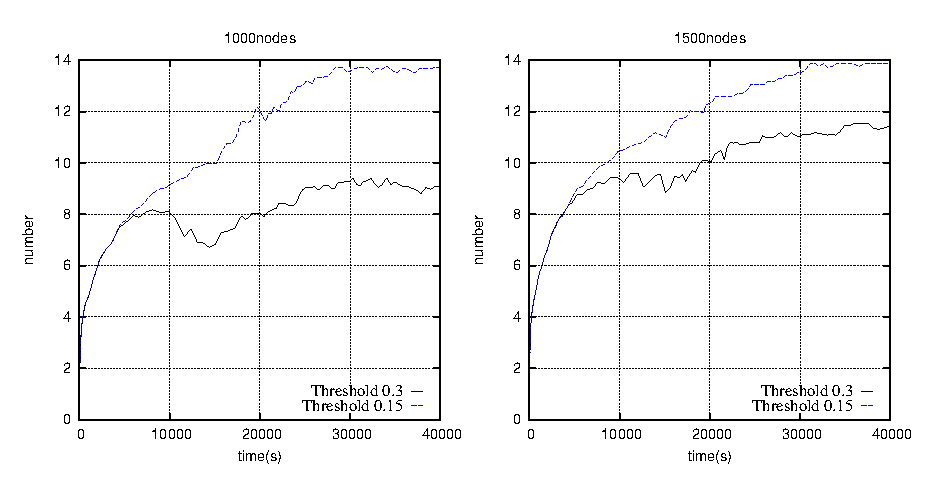
\includegraphics[width=3.5in]{figures_1/cluster_scale_with_different_threshold.eps}\\
  \caption{Average scale of clusters for different $\eta$ (left: 1,000 nodes; right: 1,500 nodes)}\label{figure_label_Scale_with_different_eta}
\end{figure}
\begin{figure}[!t]
\centering
  \includegraphics[width=3.5in]{figures_1/cluster_scale_with_different_forcast_time.eps}\\
  \caption{Average scale of clusters for different $t$ (left: 1,000 nodes; right: 1,500 nodes)}\label{figure_label_average_scale_w_t}
\end{figure}

Figure \ref{figure_label_average_scale_w_t} uses the same contact threshold $(\eta=0.3)$, but its forecast time $t$ changes from $400s$ to $200s$. In Figure \ref{figure_label_average_scale_w_t} (left), when $t=200$, the cluster scale peak value is $6.8$, and when $t=400s$, the peak reaches $9.4$. This result is due to the fact that forecast time increases the contact probability value, which causes more nodes to satisfy the clustering criteria and join clusters. Similar conclusion for the case with $1,500$ nodes (right subfigure in Figure \ref{figure_label_average_scale_w_t}).

In both cases, the curves can achieve stability after $2,000s$. It shows that the proposed clustering algorithm can cluster the network effectively and stably. Overall, the clustering phase can organize the network into clusters which have certain degree of granularity and achieve stability, which benefits the routing task inside and across the clusters in large-scale networks.

\subsection{Routing Performance}

In this set of simulations, we randomly select traces of $3,000$ vehicles from the central area ($20km \times 20km$) of Beijing. As revealed in \cite{vHuWang-23},  the central area of the city has numerous hotspot areas, which we believe is an appropriate scenario for the clustering based-routing. We investigate delivery ratio and overhead of different routing protocols under different buffer sizes. Detail parameter settings are shown in Table \ref{table_label_parameter_setting_in_ONE}.

Figure~\ref{figure_label_Delivery_ratio_w_buffersize}(a) shows that most protocols have higher delivery ratio with increased buffer size. The proposed routing algorithm yields a higher delivery ratio than the other single-strategy protocols because in such a large-scale scenario, clustering strategy groups nodes into different clusters, which makes the network more coarse-grained. As a result, from a single node's point of view, the network scale becomes much smaller. Furthermore, a node can make its forwarding decision inside or outside of the cluster more wisely which not only saves the buffer of local nodes, but also tends to the route with higher contact probability.

\begin{table}[!t]
  \centering
  \caption{Parameter setting in Simulatior ONE}\label{table_label_parameter_setting_in_ONE}
\vspace{0.1in}
  \begin{tabular}[c]{r|l}
  \hline
  Simulation Time & $10,000s$ \\
  Area & $20\times 20$ $km^{2}$ \\
  Nodes Number & $3,000$ \\
  Transmit Range& $200m$ \\
  Package Size & Random ($50,100$)k \\
  Buffer Size & [$0.5,1,\cdots,5$]M \\
  Routing Methods & CPCR ($t=400$,$\eta =0.3$), Epidemic, PRoPHET, DD \\
  \hline
  \end{tabular}
\end{table}

\begin{figure}
\centering
\begin{tabular}{cc}
  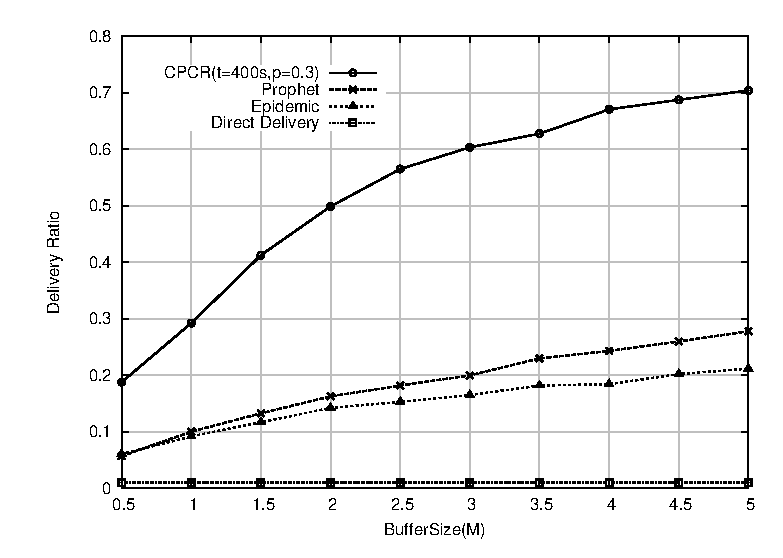
\includegraphics[width=1.5in]{figures_1/performance_deliveryrate.eps} &
   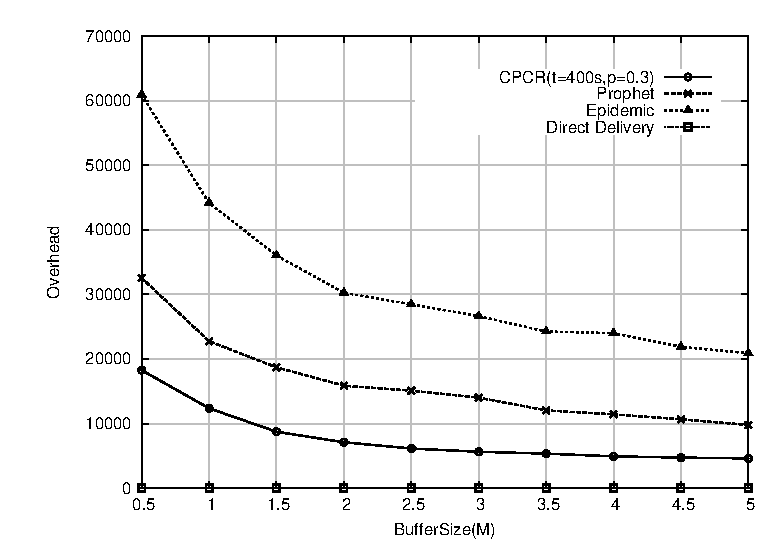
\includegraphics[width=1.5in]{figures_1/performance_overhead.eps}\\
   (a) & (b)
   \end{tabular}
  \caption{Delivery ratio and overhead of all methods with different buffer sizes}\label{figure_label_Delivery_ratio_w_buffersize}\label{figure_label_Overhead_w_buffer_sizes}
\end{figure}

Overheads are shown in Figure \ref{figure_label_Overhead_w_buffer_sizes}(b), which indicates the average number of copies generated by the network until a packet is successfully delivered. Direct Delivery is a single copy protocol which dose not produce additional copy of packets. Epidemic Protocol duplicates a copy whenever a node contact with others, thereby producing the highest overhead among the protocols. In the clustering-based routing framework, nodes generate copies only when they meet the other nodes in different clusters where no copy of the specific packet exists, thereby controlling the overhead. On the other hand, the overhead of  PROpHET Protocol is two times greater than than that of the proposed algorithm because of its high forwarding probability and one-hop decision making. As a result, the clustering-based routing algorithm yields a really low overhead between those of PROpHET and Direct Delivery Protocol, and has considerable performance in large-scale real-world urban networks.

\subsection{Scalability}

Scalability is one of the major consideration of routing protocols in large-scale DTN networks. The network scale is mainly changed by the number of nodes within the network. A greater number of nodes involved in the network indicates greater overheads since many additional copies of packets and messages to synchronous routing information are generated. In this case, the network may encounter a bottleneck and the performance of most protocols may stagnate or deteriorate. In this set of simulations, the scalability of protocols is compared by varying the number of nodes from $500$ to $3,000$. The other parameters are remaining the same as those in Table \ref{table_label_parameter_setting_in_ONE}.

\begin{figure}
\centering
\begin{tabular}{cc}
    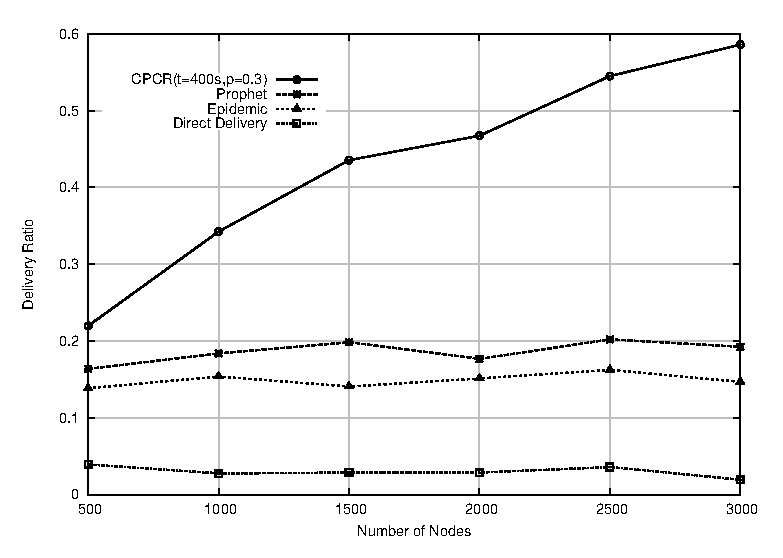
\includegraphics[width=1.5in]{figures_1/clusterScalability_delivery_radio.eps}&
     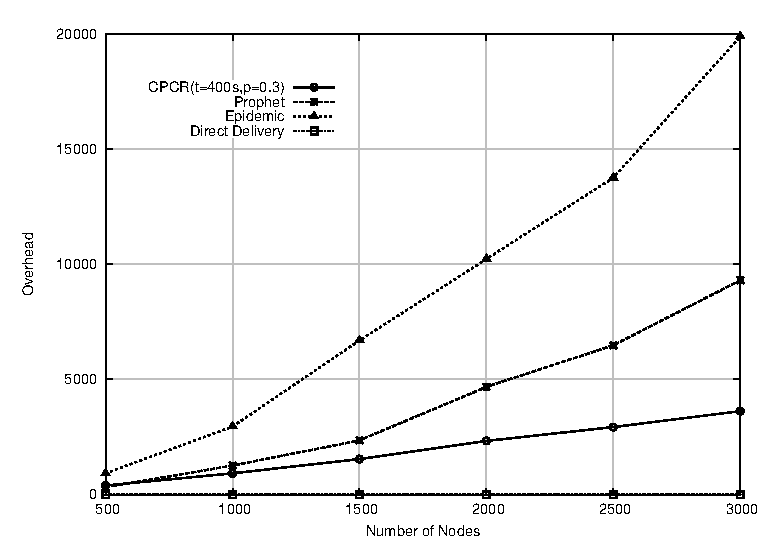
\includegraphics[width=1.5in]{figures_1/clusterScalability-overhead.eps}\\
   (a) & (b)
   \end{tabular}
    \caption{Delivery ratio and overhead of all methods with different network scales}\label{figure_label_clusterPerformance-deliveryrate}\label{figure_label_clusterPerformance-overhead}
\end{figure}

Figure \ref{figure_label_clusterPerformance-deliveryrate}(a) shows the delivery ratio in the network with different numbers of nodes. The performances of the single-strategy routing protocols do not improve as the number of nodes increases. In general, increasing nodes density can bring more contact opportunities which should lead to higher delivery ratio. However, if the network scale is large enough, the buffer capacity becomes limited during the single-strategy routing because of their overall forwarding behaviors, which limit the increase of delivery ratio. The clustering-based routing algorithm can adapt to the increasing scale. If the clustering parameters are constant $(t=400,\eta =0.3)$, the number of clusters does not change considerably when the network scale increases. Instead, the size of each cluster, which is denoted by number of nodes inside each cluster, increases. Therefore, from a single node's point of view, the buffer capacities of clusters increase. When executing inter-cluster routing, each cluster is considered a bigger ``node". Thus, the network maintains the small number of ``nodes" which have a higher buffer capacity, thereby improving routing performances.

Figure \ref{figure_label_clusterPerformance-overhead}(b) reveals the superior scalability of the proposed framework based on the other metric, namely, overhead growth rate. When the network is sparse, overhead of single-strategy protocols is close to that of clustering-based routing. However, as the number of nodes increases, overheads of those protocols, expect that of Direct Delivery, become dramatically high. On the other hand, the proposed algorithm can restrict its overhead growth rate. The reason is similar to the one we described above for delivery ratio. In large-scale urban DTNs, the proposed algorithm can help reduce network overhead and achieve scalability thereby outperforming traditional single-strategy routing protocols.

\section{Conclusion}
\label{Section6_conclusions}

In this paper, we analyzed the contact characteristics of large-scale urban DTNs over a real-world trace data set from Beijing.  Distribution of ICTs exhibits an exponential nature in such kind of urban DTN networks. To improve the scalability of routing protocols, we proposed a clustering-based routing algorithm by using contact probability estimated from ICTs distributions as the clustering metric. The extensive simulation results demonstrated that the performance and scalability of CPCR exceed those of traditional flat protocols. 




% trigger a \newpage just before the given reference
% number - used to balance the columns on the last page
% adjust value as needed - may need to be readjusted if
% the document is modified later
%\IEEEtriggeratref{8}
% The "triggered" command can be changed if desired:
%\IEEEtriggercmd{\enlargethispage{-5in}}

% references section

% can use a bibliography generated by BibTeX as a .bbl file
% BibTeX documentation can be easily obtained at:
% http://www.ctan.org/tex-archive/biblio/bibtex/contrib/doc/
% The IEEEtran BibTeX style support page is at:
% http://www.michaelshell.org/tex/ieeetran/bibtex/
%\bibliographystyle{IEEEtran}
% argument is your BibTeX string definitions and bibliography database(s)
%\bibliography{IEEEabrv,../bib/paper}
%
% <OR> manually copy in the resultant .bbl file
% set second argument of \begin to the number of references
% (used to reserve space for the reference number labels box)
%%%%\begin{thebibliography}{1}

%%%%\bibitem{IEEEhowto:kopka}
%%%H.~Kopka and P.~W. Daly, \emph{A Guide to \LaTeX}, 3rd~ed.\hskip 1em plus
 %% 0.5em minus 0.4em\relax Harlow, England: Addison-Wesley, 1999.

%%%\end{thebibliography}

\bibliographystyle{ieee}
%%  \bibliography{<your bibdatabase>}
\bibliography{cpcra}


% that's all folks
\end{document}


